\documentclass[a4paper]{scrartcl}
\usepackage{apacite}
\usepackage[english]{babel}
\usepackage[utf8]{inputenc}
\usepackage{amsmath}
\usepackage{graphicx}
\usepackage[parfill]{parskip}
\usepackage{todonotes}
\usepackage{csquotes}
\usepackage{tabularx}
\title{Master's thesis proposal}
\author{Stijn Voss, s4150511 }
\date{February 2017}
\begin{document}

\maketitle

\section{Food journaling}
Keeping track of food consumption can help for a variety of goals. For example identifying allergies, detecting deficiencies but probably most importantly achieving health and weight-loss goals. Existing applications used are MyFitnessPal\footnote{\url{https://www.myfitnesspal.com/}}, Lose It!\footnote{\url{https://www.loseit.com/}}, FatSecret\footnote{\url{https://www.fatsecret.com/}}. These applications depend on manually data entry. Either by searching in a database or scanning barcodes. 

Research shows that people tend to underestimate their calorie intake\cite{schoeller1990inaccuracies}, moreover research clearly suggests that overweight and obese people tend to underestimate caloric intake more then non-overweight people\cite{pikholz2004under, garriguet2008under}. Even more so this is true for children \cite{forrestal2011energy}. This suggests that making people aware of their caloric intake, by using food diaries,  \todo{Not sure, look for more evidence} can already help preventing overweight.\

In controlled experiments it has been shown that in general web based intervention techniques can be effective in helping people obtain healthier lifestyles.  Computer tailoring(personalized advices by a computer), expert advice or other more sophisticated behavior changing techniques results tend to increase the effectiveness \cite{lustria2009computer,kroeze2006systematic,gold2007weight,webb2010using,lustria2013meta}. More specifically it has also shown to work for diet and physical activity \cite{turner2013comparison,wharton2014dietary}

However only a small part of the people that install food diaries keep using them or achieve their goals\cite{helander2014factors} . Barriers identified include: too much effort, hard to determine portion size and which ingredients are used and loosing the habit(simply forgetting). Furthermore it was shown that users especially have difficulty tracking food that was not fast food or pre-packaged. For example home cooked meals, restaurant meals and meals prepared by friends. Other problems include: feeling guilty about eating to much and a perceived stigma around tracking(people are ashamed of their tracking behaviour when with others)  \cite{cordeiro2015barriers}. 



\section{Photo based food journaling}
To make keeping track of food diary easier researchers have been looking into photo based approaches. Where the user makes a photo of their food and this is used to estimate calories and food intake. 

One of the earliest applications is PlateMate\cite{noronha2011platemate}. Users can make a picture of their meal, using amazon machincal turk these images will then be segmented, labeled and measured. The resulting nutrition information is then shown to the user. The process is shown in figure \ref{fig:PlateMate}. When manufacturer information is taken as a baseline, the application achieves error rates comparable or better then experts that had to determine intake based on pictures. Users generally found the application easier to use than manually tracking apps. Users however felt that the application didn't work very accurately. The PlateMate system indeed seemed to over estimate the caloric intake where as users tend to underestimate, explaining the perception of being inaccurate.  \cite{schoeller1990inaccuracies}. 
\begin{figure}[h!]

\centering
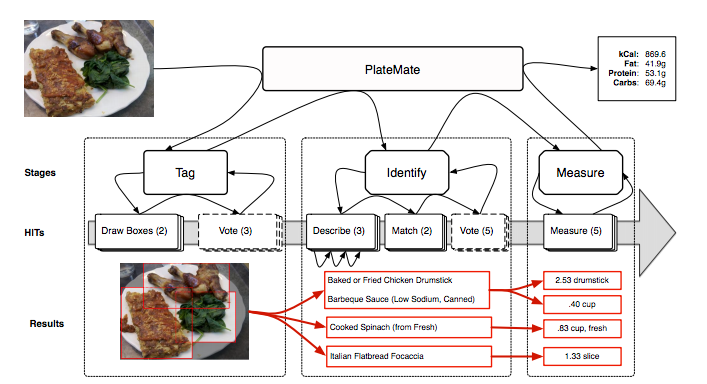
\includegraphics[scale=.4]{platemate.png}
\caption{\small{The PlateMate system. Work travels between stages and Human Intelligence Tasks (HITs) along the black
arrows, starting from the input on the left and concluding with the output on the right. The system takes submitted photos
and creates Tag tasks to annotate these photos with boxes. Each box becomes the input to a series of Identify tasks
which end with a list of foods from a commercial food database. Each individual food is then input to a Measure task,
which produces a unit and amount. Dashed boxes represent optional stages, which may be skipped during routing. Obtained from \cite{noronha2011platemate} } }
\label{fig:PlateMate}
\end{figure}
\subsection{Computer vision}
Since this is of course quit a labour-intensive way of doing food journaling, lately research focused more on using computer vision based approaches. It's often claimed that, with the raise of deep learning and convolutional neural networks, computer vision now performs on a human level. However this mainly holds for the task of object recognition. The task of food recognition seems to be more challenging.  
\begin{displayquote}
In contrast to scene classification or object detection, food typically does not exhibit any distinctive spatial layout: while we can decompose an outdoor scene with a ground plane, a horizon and a sky region, or a human as a trunk with a head and limbs, we cannot find similar patterns relating ingredients of a mixed salad. The point of view, the lighting conditions, but also (and not least) the very realization of a recipe are among the sources of high intra-class variations. On the bright side, the nature of dishes is often defined by the different colors and textures of its different local components, such that humans can identify them reasonably well from a single image, regardless of the above variations. Hence, food recognition is a specific classification problem calling for models that can exploit local information. ( \cite{bossard2014food}
\end{displayquote} \todo[inline]{This is quote from another paper, maybe not use it as such in my thesis} 
Furthermore even if we would achieve human level performance, it would probably still not be enough to accurately estimate calorie and nutrition intake. Since humans aren't always able to directly estimate all calories from a meal either, simply because it's not visible. 

Applying computer vision to the problem of food recognition is quit a new field, that shows an increase in interest lately. However the challenges, approaches and datasets differ a lot. In the following section I try to describe the different challenges and perspectives i came across in the literature. 
\subsubsection{Food/nonfood detection}
The simplest task is to try to differentiate images that contain food from images that do not. This is often solved by using a (pre-trained) convolutional neural network, and fine-tuning it on a binary classification task. Since this basically is a object recognition task performance is usually on a human level. Depending on the exact dataset and exact network, accuracy ranges from 90-99.5\% for CNN bases approaches. In table \ref{table:bg_foodnonfood_overview} a overview of different approaches is given. Please note that datasets tend to differ a bit in their very nature(some datasets count images where people are holding food as food images too). Because of this the methods are hard to compare. Furthermore most evidence suggests that fine-tuning pre-trained networks outperforms training networks from scratch. 


\begin{table}[h!]
\centering
\begin{tabularx}{\textwidth}{| X | X | X |l|}
\hline
\textbf{Paper} & \textbf{Method}(network) & \textbf{Dataset} & \textbf{Accuracy} \\ \hline
\citeA{aizawa2013food} & SVM with handcrafted features  & own & 89\%  \\ \hline
\citeA{kagaya2014food} & CNN(own)  & own(\~175,00 images from FoodLog) & 93.8\%  \\ \hline
\citeA{kagaya2015highly} &  Pre-trained CNN network in network \cite{lin2013network} & own(same as above) & 99.1\% \\ \hline
\citeA{meyers2015im2calories} & Pre-trained CNN(GoogleLeNet)  & food101 & 99.02\% \\ \hline
\citeA{singla2016food} & Pre-trained CNN(GoogleLeNet) & food5k & 99.2\% \\ \hline
\citeA{ragusa2016food} & SVM on extracted features of fine-tuned AlexNet  & UNICT-FD889, NonFood-flickr & 94.86\% \\ \hline
\citeA{bolanos2016simultaneous} & pre-trained GoogleLeNet, GAP layer in front of softmax & Constructed from Food101, ILSVRC, PASCAL & 95.64\% \\ \hline
\end{tabularx}
\caption{Overview approaches to nonfood/food classification}\label{table:bg_foodnonfood_overview}
\end{table}

\subsubsection{Food categorization}\\
Other work involves trying to classify food into a certain set of categories, however it is not obvious how these categories should be determined. Certainly not with respect to food logging. Early approaches involved determining food balance(according to the food pyramid) estimation using hand crafted features \cite{kitamura2008food}. Other approaches categorize into a limited set of food types using SVM techniques\cite{aizawa2013food} or more recently convolution neural networks \cite{meyers2015im2calories, chen2016deep}. Usually these methods can perform reasonably well by somehow limiting the number of classes. For example by just differentiating between different meals in a single restaurant \cite{beijbom2015menu} or food categories (bread, pasta, dairy etc.). An overview of different approaches is given in table \ref{table:food_cat}. \\ \\ 
Other approaches make use of the fact that food categories can be represented as a hierachical structure \cite{wu2016learning}. Food is represented in a tree structure and the task of the network is to determine the category for each tree layer. The information incorperated in the tree structure is then enforced using a random walk approach. 
\begin{table}[h!]
\centering
\begin{tabularx}{\textwidth}{| X | X | X | X |}
\hline
\textbf{Paper} & \textbf{Challenge} & \textbf{Method}  & \textbf{Performance} \\ \hline
\citeA{kitamura2008food} & Estimate food type according to food pyramid & SVM (handcrafted features) & Accuracy of 73\%    \\ \hline
\citeA{kagaya2014food} & Dataset consists of 10 different meals & CNN (own) & Accuracy of 73.70\%   \\ \hline
\citeA{chen2016deep} & Categorizing for 172 categories & VIREO Food-172 & Top-1 accuracy of 82.06\% and a top-5 accuracy of 95.88\% \\ \hline
\end{tabularx}
\caption{Overview of different challenges and methods in food categorization tasks }
\label{table:food_cat}
\end{table}\\
\subsubsection{Recipe retrieval}
Using categorization to recognize different meals can be very difficult since there might be possibly 10's of thousand categories. \citeA{chen2016deep} noted that instead of focusing on trying to find the dish directly by a picture, trying to to estimate the ingredients might be easier. Please note that their paper is mainly focused on the Chinese cuisine, where dishes often involve small portions with few ingredients(which are often pretty recognizable). 

Based on a pre-trained VGG16 network they trained a multi-task deep neural network that had to predict the ingredients and the category of the dish. For the categorization task they achieved a top-1 accuracy of 82.06\% and a top-5 accuracy of 95.88\%(out of 172 categories). 

The ingredients are predicted using a multi-label output layer with sigmoid activation. A conditional random field is used to account for inter-ingredient dependencies.   For the ingredients they achieve a micro-F1 of 67.17\% and a macro-f1 of 47.18\%. It is clearly shown that the multi-task approach significantly increases their performance. 

They also provided the network with images of recipes that the network had never seen before. Given the resulting ingredient probabilities for every recipes a score was then determined using eq \ref{eq1}. \begin{equation}
    S_i = \sum_{c \in O \cap c \in Q_i } x_c
    \label{eq1}
\end{equation}
Where O contains the ingredients of the recipe, $Q_i$ contains the ingredients found in the network and $X_c$ contains the probability for that ingredient. The network was able to predict the right recipe in the top-10 for about 50\% of the cases. \\ \\


In their next paper they extended their method with the concept of Stacked attention networks(SAN) \cite{yang2016stacked}. SAN's are original introduced to tackle the challenge of answering questions that are related to the content of an image for example `what is the color of the horns?'. A SAN uses the last features of a convolutional network where spatial information is still intact, just before the fully connected layers. Given the semantic representation of a query and the spatial features, a attention area is selected and a new query if formulated . They authors claim that this represents the normal reasoning process required behind such question. First search the horns and put your attention to this area, next determine the color. 

\citeA{chen2017cross} use the same idea but then try to locate the ingredients on a picture. The semantic information of the question is replaces by a vector representing the ingredients of the meal. The network job is to locate the ingredients. \todo[inline]{I don't entirely understand their method. I don't understand their objective function and don't understand how they get actual ingredients from a to classify image. Since they use both the image and ingredients as input during training. \\ \\ Furthermore i am not sure about their method either. Finding ingredients doesn't really seem to reflect a reasoning process.} 

\subsubsection{Localization and segmentation}
Another important aspect of computer vision for food seems to be locating food on a picture or segment if multiple food objects are being displayed in a picture. \citeA{bolanos2016simultaneous} make use of foon/non-food classification network to address the challenge of food localization and segmentation. They used the GoogleLeNet network, replaced the last layers with a `Global average pooling(GAP)`-layer such that spatial information is not lost. Using softmax they then fine-tuned the network on the binary food/nonfood identification task. Using the output from the GAP layer they now could create a food activation map for the image, indicating a probability of food being present for each pixel. This can then be used to draw bounding boxes.  Testing the performance with a minimum IoU(intersection over union) of .5 to test each bounding box on the UECFood256 and EgocentricFood datasets they found a accuracy of 36.84\% and 6.41\% respectively.  

\citeA{meyers2015im2calories} noted that instead of using bounding boxes it is better to use segmentation. Since food tend not to be rectangular in nature. They made use of  the DeepLab\cite{chen2014semantic} method. They achieve an accuracy of 76\% and an average IoU of .25 on the Food101-segmented dataset.   
\todo[inline]{I don't understand the DeepLab paper however \cite{noh2015learning} seem to be an improvement of that paper and i do  understand that one. }

\subsubsection{Quantity estimation}
Another important aspect of food logging is of course the volume of the meal. \citeA{meyers2015im2calories} did this by first predicting the pixel depth for each pixel using a CNN based on a simple RGB input image \cite{eigen2015predicting}. They achieve an average error of 18 centimeters. Based on this they create a 3d voxel grid of 2mmx2mm each(where they used the average predicted height as height for each voxel), with respect to the surface(which they detect). By re-using the segmentation task they could then try to estimate the volume of the meal. The error differs a lot between the different meal classes. For most of the meal classes the volume error stayed below an average of 200ml. 

\subsubsection{Context}
Even with human level performance it would difficult to estimate the exact meal or food presented, so incorporating contextual knowledge seems crucial. \citeA{aizawa2013food} used a Bayesian method to estimate food balance(according to the food pyramid) and incorporated user knowledge using priors.  Other approaches assumed that the restaurant a user was visiting was known and limited the search space down this way \cite{joutou2009food}. \citeA{meyers2015im2calories} trained a separate CNN network per restaurant.
\subsubsection{Constant monitoring vs user photo}
Research also makes a distinction between constant monitoring and pictures made by user. Wearable cams worn around the neck could constantly track what one is eating or even prepares while cooking \cite{o2013using, liu2012intelligent,jia2014accuracy}. This could lead to less effort for the user and more accurate tracking, but also is technically way more challenging. 
\todo[inline]{Mobile device/platform}
\cite{horiguchi2016log}

\newpage
\section{Proposal}
Since the litarature suggests that recognizing prepared meals is cause for the most difficulties i want to address that problem first. The problem of food categorization is difficult since the same category can have a lot of different spatial properties(the same meal or food doesn't always look the same, but sometimes it does) as compared to other visual tasks. Your model has to be invariant to these spatial features. Furthermore you need a large amount of categories in order to be useful, quickly leading to over-fitting certain of these specific spatial features. In short I can think of two ways that can help tackle this. 
\begin{itemize}
\item Use more training data(especially more per category)
\item Make your model less vulnerable  to these spatial features anyway. Most models that i have seen fine-tune existing object recognition networks, which might be a disadvantage. Furthermore the network architecture itself might also be a problem. \todo[inline]{Very speculative, should do more research}
\end{itemize}

The recipe retrieval concept of \cite{chen2016deep} seems very promising since, by predicting ingredients, they reduce the categories required and prevent having to define these categories. And thus the model will learn to be invariant more quickly. However I think it has some limitations. First of all if you try to recognize meals by just the ingredients you might lose quit some information that could help you predict the right meal. For example the relative ratio between ingredients or shapes of ingredients might actually tell us something about the actual meal. Furthermore the way they query for recipes now seems to require to calculate the distance to each recipe separately which can be too time consuming if you have lot's of recipes\todo[]{Not very sure about this, also not really sure if my approach would improve on it}. Another disadvantage is that they not take into account that some ingredients will never be visible and actually might be quit important for caloric intake(for example: sugar, oils). Such ingredients will always have to inferred from something else: for example by asking the user or using context information.

Instead I propose to model meals in a vector space(`recipe space`) that represents the relevant(for food logging) information for that meal. Analogous to representing the semantics of words in a vector space using word embeddings. \todo[]{Look up some papers that do something like this, for other problems}. To make sure this vector does contain only relevant information. I would let the network predict metrics that are relevant for food journals. For example:
\begin{itemize}
    \item Ingredient and it's ratio prediction (it might also help to only predict ingredients that can be predicted by using vision)
    \item category prediction(to make sure meals of different categories, with similar ingredients are not mapped to the same vector space) 
    \item Calorie(density) prediction
\end{itemize}

By forcing the network to go trough a small enough layer, before predicting the above classes and metrics, and using the activations of that layer. A vector  could be created that contains all information that is required to predict these metrics for each picture of meal. Similar meals should then have a small distance to each other, where as un-similar meals would have a larger distance. Meals that are difficult to separate based on vision should also have a smaller distance. 

Creating a vector space might seem a bit far fetched but i believe it would overcome the need to categorize food in finite set of categories, while still using all information that identifies a meal. In practice it might also allow to query for something like this: find recipes that lay close to this "visual recipe space" but have very different "invisible" ingredients? Providing a user with a set of options. 

The research question I want to answer is: Can we represent meals in a vector space?

\subsection{Approach}
\textbf{Dataset} \\ 
Using the schema.org structured recipe format\footnote{\url{http://schema.org/Recipe}} combined with the common crawl\footnote{\url{http://commoncrawl.org/}} index I could obtain a very large dataset from a lot of sources that contain a huge variety of meals. The recipe format provides in a lot of different properties like ingredients, nutrition information and a image.  However the properties are not always perfectly clean and probably need some additional processing. For example ingredients come with quantities and forms. Calories are defined for the whole meal or per serving etc. It could be interesting to try to apply word2vec on ingredients(like similar words will be used in the same context, same ingredients will be used in the same context). Double ingredients could than be found by looking for very similar vectors analogous to finding different spelling alternatives using word2vec values in NLP tasks.

An alternative approach could be to write a site specific scraping script by hand for a website and use these. However using the schema.org approach might be useful since it can be handy in a real practical application. For example logging your meal by providing an url could be a relatively easy and useful feature. Information about how to use a wide variety of web sources can be useful. 
\\ \\
\textbf{General steps}\\
Once I have a dataset I would start by re-using an existing network(like GoogleNet, this one seems to be successful in other papers). Remove the last layers and replace it with my multi-task layers. First i could train it without fine-tuning the first layers, speeding up the process. This would allow me to find out what the dimensions of the recipe space could work and determine other parameters/choices. Later on i could try to improve my performance by fine-tuning or using other architectures etc. 

\textit{One open question is how to evaluate my method..?}


\section{Appendix}
\subsection{Datasets}

While reading the papers I came across a lot of datasets. I sum them up here for later reference. 
\begin{itemize}
\item \textbf{Food101} Contains 101,000 images of 101 different meals/categories. Taken from \url{foodspotting.com} \url{http://www.vision.ee.ethz.ch/datasets/food-101/.} \cite{bossard2014food}
\item \textbf{UEC-FOOD-100} Contains 9060 images of 100 categories mainly japanese recipes. Focused on so called multi-food meals. \cite{matsuda2012recognition}
\item \textbf{UEC-FOOD-256} 256 food categories, extension of UEC-FOOD-100. Build by searching for the original categories on flickr and instagram. Based on first dataset, check if indeed food and assign some category. Using crowdsourcing improve further\todo{Not entirely clear to me what they did, but not so relevant now} \cite{kawano2014automatic}
\item \textbf{FID  dataset} obtained by looking for the \#food tag on instagram manually labeled. Resulting in 4,230
food images and 5,428 non-food images. Based on a small sub sample it seems that this dataset hash quit a broad definition of food images. Some food images contain humans as the main topic while enjoying food. These images are labeled as food images. \cite{kagaya2015highly}
\item \textbf{food 5k and 11k} These data-sets where assembled using the  Food101 datasets and UEC-FOOD-* datasets. 5k is focused on non-food/food classification, 11k divides the images into 11 categories. Optionally some images from social media where added \cite{singla2016food} \url{http://mmspg.epfl.ch/food-image-datasets}
\item \textbf{VIREO Food-172}  \cite{chen2016deep} 110,241 images divided into 172 chinese food categories and assigned an average of 3 ingredients per recipe out of 353 possibles recipes. \url{}
\item \textbf{UNICT-FD889} 3583 images of 889 different plates \cite{farinella2014benchmark} \url{http://iplab.dmi.unict.it/UNICT-FD889/}
\item \textbf{Flickr-Food, FlickrNonFood}  Obtained from flickr and manually labeld 4805 of food and 8005 not food \cite{farinella2015exploitation} \url{http://iplab.dmi.unict.it/madima2015/}
\item \textbf{EgocentricFood} contains images from a wearable cam \cite{bolanos2016simultaneous} \url{http://www.ub.edu/cvub/egocentricfood/}
\end{itemize}

\newpage
\bibliographystyle{apacite}
\bibliography{bib}
\end{document}
